
\documentclass[letterpaper,hide notes,xcolor={table,svgnames},pdftex,10pt]{beamer}
\def\showexamples{t}

\usecolortheme{crane}
\setbeamertemplate{navigation symbols}{}

\usetheme{MyPittsburgh}
\usepackage{hyperref}
\usepackage{graphicx,xspace}
\usepackage[normalem]{ulem}
\usepackage{multicol}
\usepackage{amsmath,amssymb,amsthm,graphicx,xspace}
\newcommand\SF[1]{$\bigstar$\footnote{SF: #1}}

\usepackage[sfdefault,lf]{carlito}
\usepackage[T1]{fontenc}
\usepackage[scaled]{beramono}
\usepackage{tikzpagenodes}
\newcommand{\Rplus}{\protect\hspace{-.1em}\protect\raisebox{.35ex}{\small{\small\textbf{+}}}}
\newcommand{\Cpp}{\mbox{C\Rplus\Rplus}\xspace}

\newcounter{tmpnumSlide}
\newcounter{tmpnumNote}

\newcommand\mnote[1]{%
	\addtocounter{tmpnumSlide}{1}
	\ifdefined\showcues {~\tiny\fbox{\arabic{tmpnumSlide}}}\fi
	\note{\setlength{\parskip}{1ex}\addtocounter{tmpnumNote}{1}\textbf{\Large \arabic{tmpnumNote}:} {#1\par}}}

\newcommand\mmnote[1]{\note{\setlength{\parskip}{1ex}#1\par}}


\newcommand\mquestion[2]{{~\color{red}\fbox{?}}\note{\setlength{\parskip}{1ex}\par{\Large \textbf{?}} #1} \note{\setlength{\parskip}{1ex}\par{\Large \textbf{A}} #2\par}\ifdefined \presentationonly \pause \fi}

\newcommand\blackboard[1]{%
	\ifdefined   \showblackboard
		{#1}
	\else {\begin{center} \fbox{\colorbox{blue!30}{%
						\begin{minipage}{.95\linewidth}%
							\hspace{\stretch{1}} Some space intentionally left blank; done at the blackboard.%
						\end{minipage}}}\end{center}}%
	\fi%
}

\usepackage{listings}
\lstset{%
	keywordstyle=\bfseries,
	aboveskip=15pt,
	belowskip=15pt,
	captionpos=b,
	identifierstyle=\ttfamily,
	frame=lines,
	numbers=left, basicstyle=\scriptsize, numberstyle=\tiny, stepnumber=0, numbersep=2pt}

\usepackage{siunitx}
\newcommand\sius[1]{\num[group-separator = {,}]{#1}\si{\micro\second}}
\newcommand\sims[1]{\num[group-separator = {,}]{#1}\si{\milli\second}}
\newcommand\sins[1]{\num[group-separator = {,}]{#1}\si{\nano\second}}
\sisetup{group-separator = {,}, group-digits = true}

%% -------------------- tikz --------------------
\usepackage{tikz}
\usetikzlibrary{positioning}
\usetikzlibrary{arrows,backgrounds,automata,decorations.shapes,decorations.pathmorphing,decorations.markings,decorations.text}

\tikzstyle{place}=[circle,draw=blue!50,fill=blue!20,thick, inner sep=0pt,minimum size=6mm]
\tikzstyle{transition}=[rectangle,draw=black!50,fill=black!20,thick, inner sep=0pt,minimum size=4mm]

\tikzstyle{block}=[rectangle,draw=black, thick, inner sep=5pt]
\tikzstyle{bullet}=[circle,draw=black, fill=black, thin, inner sep=2pt]

\tikzstyle{pre}=[<-,shorten <=1pt,>=stealth',semithick]
\tikzstyle{post}=[->,shorten >=1pt,>=stealth',semithick]
\tikzstyle{bi}=[<->,shorten >=1pt,shorten <=1pt, >=stealth',semithick]

\tikzstyle{mut}=[-,>=stealth',semithick]

\tikzstyle{treereset}=[dashed,->, shorten >=1pt,>=stealth',thin]

\usepackage{ifmtarg}
\usepackage{xifthen}
\makeatletter
% new counter to now which frame it is within the sequence
\newcounter{multiframecounter}
% initialize buffer for previously used frame title
\gdef\lastframetitle{\textit{undefined}}
% new environment for a multi-frame
\newenvironment{multiframe}[1][]{%
	\ifthenelse{\isempty{#1}}{%
		% if no frame title was set via optional parameter,
		% only increase sequence counter by 1
		\addtocounter{multiframecounter}{1}%
	}{%
		% new frame title has been provided, thus
		% reset sequence counter to 1 and buffer frame title for later use
		\setcounter{multiframecounter}{1}%
		\gdef\lastframetitle{#1}%
	}%
	% start conventional frame environment and
	% automatically set frame title followed by sequence counter
	\begin{frame}%
		\frametitle{\lastframetitle~{\normalfont(\arabic{multiframecounter})}}%
		}{%
	\end{frame}%
}
\makeatother

\makeatletter
\newdimen\tu@tmpa%
\newdimen\ydiffl%
\newdimen\xdiffl%
\newcommand\ydiff[2]{%
	\coordinate (tmpnamea) at (#1);%
	\coordinate (tmpnameb) at (#2);%
	\pgfextracty{\tu@tmpa}{\pgfpointanchor{tmpnamea}{center}}%
	\pgfextracty{\ydiffl}{\pgfpointanchor{tmpnameb}{center}}%
	\advance\ydiffl by -\tu@tmpa%
}
\newcommand\xdiff[2]{%
	\coordinate (tmpnamea) at (#1);%
	\coordinate (tmpnameb) at (#2);%
	\pgfextractx{\tu@tmpa}{\pgfpointanchor{tmpnamea}{center}}%
	\pgfextractx{\xdiffl}{\pgfpointanchor{tmpnameb}{center}}%
	\advance\xdiffl by -\tu@tmpa%
}
\makeatother
\newcommand{\copyrightbox}[3][r]{%
	\begin{tikzpicture}%
		\node[inner sep=0pt,minimum size=2em](ciimage){#2};
		\usefont{OT1}{phv}{n}{n}\fontsize{4}{4}\selectfont
		\ydiff{ciimage.south}{ciimage.north}
		\xdiff{ciimage.west}{ciimage.east}
		\ifthenelse{\equal{#1}{r}}{%
			\node[inner sep=0pt,right=1ex of ciimage.south east,anchor=north west,rotate=90]%
			{\raggedleft\color{black!50}\parbox{\the\ydiffl}{\raggedright{}#3}};%
		}{%
			\ifthenelse{\equal{#1}{l}}{%
				\node[inner sep=0pt,right=1ex of ciimage.south west,anchor=south west,rotate=90]%
				{\raggedleft\color{black!50}\parbox{\the\ydiffl}{\raggedright{}#3}};%
			}{%
				\node[inner sep=0pt,below=1ex of ciimage.south west,anchor=north west]%
				{\raggedleft\color{black!50}\parbox{\the\xdiffl}{\raggedright{}#3}};%
			}
		}
	\end{tikzpicture}
}


%% --------------------

%\usepackage[excludeor]{everyhook}
%\PushPreHook{par}{\setbox0=\lastbox\llap{MUH}}\box0}

%\vspace*{\stretch{1}

%\setbox0=\lastbox \llap{\textbullet\enskip}\box0}

\setlength{\parskip}{\fill}

\newcommand\noskips{\setlength{\parskip}{1ex}}
\newcommand\doskips{\setlength{\parskip}{\fill}}

\newcommand\xx{\par\vspace*{\stretch{1}}\par}
\newcommand\xxs{\par\vspace*{2ex}\par}
\newcommand\tuple[1]{\langle #1 \rangle}
\newcommand\code[1]{{\sf \footnotesize #1}}
\newcommand\ex[1]{\uline{Example:} \ifdefined \presentationonly \pause \fi
	\ifdefined\showexamples#1\xspace\else{\uline{\hspace*{2cm}}}\fi}

\newcommand\ceil[1]{\lceil #1 \rceil}


\AtBeginSection[]
{
	\begin{frame}
		\frametitle{Outline}
		\tableofcontents[currentsection]
	\end{frame}
}



\pgfdeclarelayer{edgelayer}
\pgfdeclarelayer{nodelayer}
\pgfsetlayers{edgelayer,nodelayer,main}

\tikzstyle{none}=[inner sep=0pt]
\tikzstyle{rn}=[circle,fill=Red,draw=Black,line width=0.8 pt]
\tikzstyle{gn}=[circle,fill=Lime,draw=Black,line width=0.8 pt]
\tikzstyle{yn}=[circle,fill=Yellow,draw=Black,line width=0.8 pt]
\tikzstyle{empty}=[circle,fill=White,draw=Black]
\tikzstyle{bw} = [rectangle, draw, fill=blue!20,
text width=4em, text centered, rounded corners, minimum height=2em]

\newcommand{\CcNote}[1]{% longname
	This work is licensed under the \textit{Creative Commons #1 3.0 License}.%
}
\newcommand{\CcImageBy}[1]{%
	\includegraphics[scale=#1]{creative_commons/cc_by_30.pdf}%
}
\newcommand{\CcImageSa}[1]{%
	\includegraphics[scale=#1]{creative_commons/cc_sa_30.pdf}%
}
\newcommand{\CcImageNc}[1]{%
	\includegraphics[scale=#1]{creative_commons/cc_nc_30.pdf}%
}
\newcommand{\CcGroupBySa}[2]{% zoom, gap
	\CcImageBy{#1}\hspace*{#2}\CcImageNc{#1}\hspace*{#2}\CcImageSa{#1}%
}
\newcommand{\CcLongnameByNcSa}{Attribution-NonCommercial-ShareAlike}

\newenvironment{changemargin}[1]{% 
	\begin{list}{}{% 
		\setlength{\topsep}{0pt}% 
		\setlength{\leftmargin}{#1}% 
		\setlength{\rightmargin}{1em}
		\setlength{\listparindent}{\parindent}% 
		\setlength{\itemindent}{\parindent}% 
		      \setlength{\parsep}{\parskip}% 
		      }% 
		\item[]}{\end{list}}




\title{Lecture 17 --- Real-Time Scheduling}

\author{Jeff Zarnett \\ \small \texttt{jzarnett@uwaterloo.ca}}
\institute{Department of Electrical and Computer Engineering \\
  University of Waterloo}
\date{\today}


\begin{document}

\begin{frame}
  \titlepage

 \end{frame}
 
\begin{frame}
\frametitle{Real-Time Scheduling}


\begin{center}
	
\includegraphics[width=0.7\textwidth]{images/tiktok.jpg}
\end{center}

\end{frame}

\begin{frame}
\frametitle{Real-Time Scheduling}

Real-Time scheduling is just scheduling for real-time systems.

But what is a real-time system?

Supposed to respond to events within some real (wall-clock) time. 

There are deadlines, and there are consequences for missing deadlines. 

Fast is not as important as predictable.

\end{frame}

\begin{frame}
\frametitle{Task Management}

The term \alert{task} is used to refer to something that needs doing.

Yes, the scheduler operates on threads rather than specific things to do.

Let's say each task corresponds to a thread trying to some work.

\end{frame}

\begin{frame}
\frametitle{Task Types}

\begin{center}
	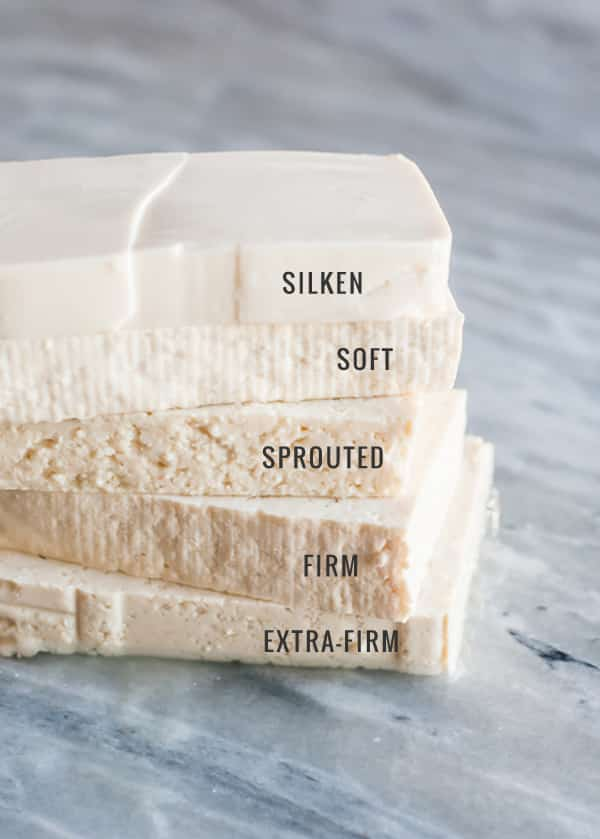
\includegraphics[width=0.4\textwidth]{images/tofu.jpg}
\end{center}

Not quite... Hard, Firm, Soft.

\end{frame}

\begin{frame}
\frametitle{Hard and Soft Real-Time}

\alert{Hard real-time}: it has a deadline that must be met to prevent an error, prevent some damage to the system, or for the answer to make sense. 

If a task is attempting to calculate the position of an incoming missile, a late answer is no good. 

A \alert{soft real-time} task has a deadline that is not, strictly speaking, mandatory; missing the deadline degrades the quality of the response, but it is not useless.

\end{frame}

\begin{frame}
\frametitle{Firm}

Firm is about severity of consequences. 

A firm deadline is one in which the response is useless if it arrives a little too late.

A hard deadline is one in which the system itself fails if it doesn't meet the deadline.
\end{frame}

\begin{frame}
\frametitle{Desktop OSes and Real-Time}

Most of the operating systems you are familiar with (standard Desktop/Server Linux, Mac OS, Windows) are not very suitable to real time systems. 

They make few guarantees, if any, about service. 

When there are consequences for missing deadlines, this kind of thing matters. 

\end{frame}


\begin{frame}
\frametitle{Userspace?}

Remember Java's ``stop the world'' garbage collector scenario.

Why is the OS not suitable for real-time operations?

\end{frame}

\begin{frame}
\frametitle{Arbitrary Timelines}

How long does it take to run a system call?

If you measure it, is that the average scenario? Worst-case?

Interrupts? Concurrency-control mechanisms?

\end{frame}

\begin{frame}
\frametitle{It's Different}

\begin{center}
	
\includegraphics[width=0.4\textwidth]{images/thinkdifferent.png}
\end{center}

Much of the difference of real-time systems is in scheduling.

\end{frame}

\begin{frame}
\frametitle{Hard Real-Time Failure}

If a task is hard real-time, there are two scenarios in which it might not complete before its deadline. 

The first is that it is scheduled too late; like an assignment that will take two hours to complete being started one hour before the deadline. 

\begin{center}
	
\includegraphics[width=0.4\textwidth]{images/notime.jpg}
\end{center}

\end{frame}

\begin{frame}
\frametitle{Hard Real-Time Failure}

If that is the case, the system will likely reject the request to start the task, or perhaps never schedule the task to run at all. 

Why waste computation time on a task that will not finish in time? 

... Could it have been completed if scheduled better?

\end{frame}

\begin{frame}
\frametitle{Hard Real-Time Failure}

The second scenario is that at the time of starting, completion was possible. 

For whatever reason (e.g., other tasks with higher priority have occurred) it is no longer possible to meet the deadline. 

\end{frame}

\begin{frame}
\frametitle{Hard Real-Time Failure}

In that case, execution of the task may be terminated partway through so that no additional effort is wasted on a task that cannot be completed.

... Could this task have been completed if scheduled better?

\end{frame}

\begin{frame}
\frametitle{Properties of Real-Time Systems}

Real-time systems are considered to be unique in five key areas:

\begin{enumerate}
	\item Determinism
	\item Responsiveness
	\item User (administrator) control
	\item Reliability
	\item Fail-Soft operation
\end{enumerate}


\end{frame}

\begin{frame}
\frametitle{Determinism}

\begin{center}
	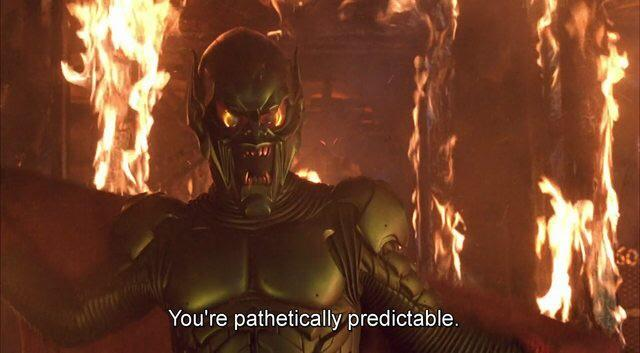
\includegraphics[width=0.4\textwidth]{images/predictable.jpg}
\end{center}

Determinism: operations are predictable.

Perfect determinism probably won't happen; just need guarantees.

\end{frame}

\begin{frame}
\frametitle{Nondeterminism?}

Nondeterminism isn't necessarily bad: e.g., caching.

The presence of caching makes the worst case no worse and the best case much better -- this sounds like free performance to me! 

Can you think of something else?

\end{frame}

\begin{frame}
\frametitle{Responsiveness}

\begin{center}
	
\includegraphics[width=0.4\textwidth]{images/notresponding.jpg}
\end{center}

Responsiveness includes not only the time to execute the interrupt handler...

Also the time it takes to start the interrupt handler and what happens if the interrupt is itself interrupted by another higher-priority interrupt.

\end{frame}

\begin{frame}
\frametitle{Administrator Control}

\begin{center}
	
\includegraphics[width=0.4\textwidth]{images/twup.png}
\end{center}

Administrator control could be much less or much more!

Typical OS is somewhere in between.

\end{frame}

\begin{frame}
\frametitle{Reliability \& Fail-Soft}

\begin{center}
	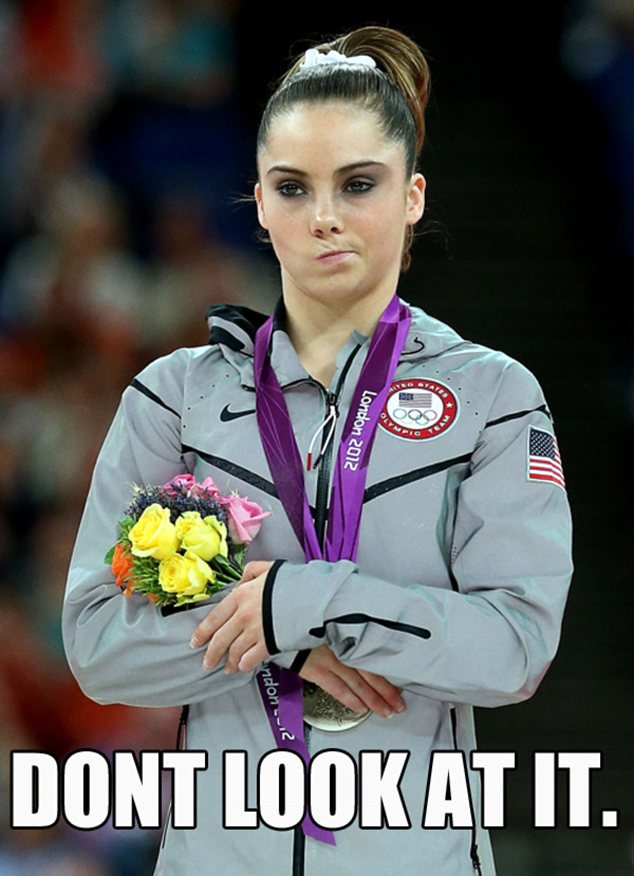
\includegraphics[width=0.4\textwidth]{images/silvermedal.jpg}
\end{center}


Fail-soft: do our best even if it's not possible to succeed at all tasks.

\end{frame}

\begin{frame}
\frametitle{Scheduling is Central}

\begin{center}
	
\includegraphics[width=\textwidth]{images/captainschair.jpg}
\end{center}

\end{frame}

\begin{frame}
\frametitle{Scheduling Algorithm Selections}

Choosing the wrong algorithm guarantees failure.

Scheduling algorithms we've discussed so far are inadequate.

Fairness and minimizing average response time are irrelevant.

\end{frame}

\begin{frame}
\frametitle{Stay On Target!}
The goal is to make sure hard real-time tasks complete.\\
\quad And as many as possible of the soft real-time tasks.

Right algorithm? Success is possible but not guaranteed.

\begin{center}
	
\includegraphics[width=0.4\textwidth]{images/physics.jpg}
\end{center}

\end{frame}

\begin{frame}
\frametitle{Preemption is the Priority}

Non-preemptive algorithms won't work here.

Immediate preemption makes sense.

Why, when we can make timeslices super small?

\end{frame}

\begin{frame}
\frametitle{What Kind of Tasks?}

Every task can be categorized as one of the four kinds:

\begin{enumerate}
	\item Fixed-Instance
	\item Periodic
	\item Aperiodic
	\item Sporadic
\end{enumerate}

\end{frame}

\begin{frame}
\frametitle{Fixed Instance}

\begin{center}
	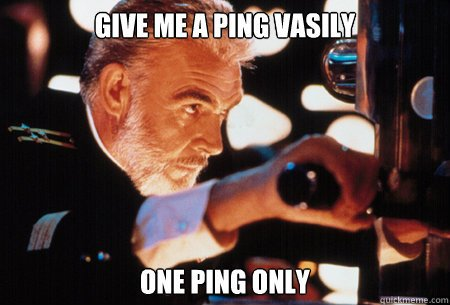
\includegraphics[width=0.4\textwidth]{images/oneping.jpg}
\end{center}

This kind of task happens only a fixed number of times (usually once).

\end{frame}

\begin{frame}
\frametitle{Periodic Tasks}

\begin{center}
	
\includegraphics[width=0.4\textwidth]{images/periodic.jpg}
\end{center}

If a task repeats at regular intervals, it's \alert{periodic}.

\end{frame}

\begin{frame}
\frametitle{Periodic Tasks}

Periodic tasks have two relevant attributes:\\
\quad: $\tau_{k}$, the period; \\
\quad $c_{k}$, the worst-case computation time

We can calculate the utilization of periodic tasks:

\begin{center}
$U = \sum\limits_{k=1}^n\dfrac{c_{k}}{\tau_{k}}$
\end{center}

\end{frame}

\begin{frame}
\frametitle{Overloaded}

If $U > 1$, it means the system is overloaded: there are too many periodic tasks. 

We cannot guarantee that the system can execute all tasks and meet the deadlines.

\begin{center}
	
\includegraphics[width=0.4\textwidth]{images/allshesgot.jpg}
\end{center}

Otherwise, we can devise a schedule.

\end{frame}

\begin{frame}
\frametitle{Only Periodic?}

If the only tasks in the system are periodic ones, then we can create a fixed schedule for them.

Example: classes at UW.

But life is rarely so nice.

\end{frame}

\begin{frame}
\frametitle{Aperiodic Tasks}

Aperiodic tasks occur irregularly with no minimum interval.

\begin{center}
	
\includegraphics[width=0.4\textwidth]{images/aperiodic.jpg}
\end{center}

If we expect an average arrival rate of 3 requests per second, there is still a 1.2\% chance that eight or more requests appear within 1~second

\end{frame}

\begin{frame}
\frametitle{Sporadic Task}

Sporadic tasks are aperiodic, but they require meeting deadlines.

\begin{center}
	
\includegraphics[width=0.3\textwidth]{images/sporadic.jpg}
\end{center}

We need a guarantee that there is a minimum time $\tau_{k}$ between occurrences of the event.

They can overload the system?

\end{frame}

\begin{frame}
\frametitle{Estimation}

Where do task execution times come from?

\begin{center}
	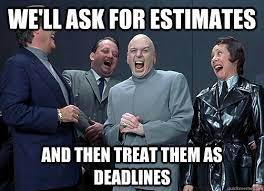
\includegraphics[width=0.5\textwidth]{images/estimates.jpg}
\end{center}

\end{frame}

\begin{frame}
\frametitle{Worst Case Scenario}

We always assume the worst case scenario! 

There's two ways to do it: source code analysis and empirical testing.

Err on the side of caution... More money? Worse battery life?

\end{frame}

\begin{frame}
\frametitle{Airline Example}

\begin{center}
	
\includegraphics[width=0.5\textwidth]{images/cancelled-flights.jpg}
\end{center}

Caused by lack of capacity...

\end{frame}

\begin{frame}
\frametitle{Code Analysis}

Code analysis is exactly what it sounds like.

Try to figure out how long the execution takes on the longest path.

Overestimate; ignores pipelining and compiler optimizations...

\end{frame}

\begin{frame}
\frametitle{Estimation is Hard}

\begin{center}
	
\includegraphics[width=0.4\textwidth]{images/nasa-logo.png}
\end{center}

NASA/JPL Guidelines:
\begin{enumerate}
	\item No recursion and no \texttt{goto}
	\item Loops must have a fixed bound
	\item No dynamic memory allocation after init
\end{enumerate}

\end{frame}

\begin{frame}
\frametitle{Empirical Observation}

If you already have a version $n$ of the system and want to build version $n+1$: extrapolate?

Otherwise, simulate.

Simulation must be representative or misleading.

\end{frame}

\begin{frame}
\frametitle{Confidence Intervals}

It's possible to estimate using known mathematical techniques the worst case runtime with the \alert{confidence interval}.

We might say that the maximum time is $t$ with 99\% confidence, based on the standard deviation.

\end{frame}

\begin{frame}
\frametitle{Ready to Schedule Some?}

Now that we understand real-time systems and classification...

Let's actually schedule some!

\end{frame}


\end{document}

